%%%%%%%%%%%%%%%%%%%%%%%%%%%%%%%%%%%%%%%%%%%%%%
%       Plantilla Informes Isaias Cardenas
%%%%%%%%%%%%%%%%%%%%%%%%%%%%%%%%%%%%%%%%%%%%%%

\documentclass[letterpaper,12pt]{report}
\usepackage[right=2cm,left=3cm,top=2cm,bottom=2cm,footskip=1.4cm]{geometry}%margenes de la pagina

\usepackage{ucs}
\usepackage[utf8x]{inputenc}
\usepackage[spanish, es-tabla]{babel}
\usepackage[T1]{fontenc}
\usepackage{blindtext}
\usepackage{enumitem}
\usepackage{graphicx}
\usepackage{listings} % escribir codigo
\usepackage{algpseudocode} % escribir algoritmos
\graphicspath{ {./images/} }
\usepackage{multicol} % multicolumnas
% \usepackage{subfigure} % incluir multiples imágenes en una figura
\usepackage{float} % poscicionar imagenes
% \fontfamily{ppl}\selectfont % change font

% \RequirePackage{hyperref}
% \RequirePackage{url} %citacion de URL
% \usepackage{hyperref}
\linespread{1.5} %interlineado

%borra la palabra "capitulo"
\usepackage{titlesec}
\titleformat{\chapter}[display]
    {\normalfont\huge\bfseries}{}{0pt}{\Huge}
\titlespacing*{\chapter}
    {0pt}{10pt}{40pt}

\setlength\parindent{0pt} %tamaño indentacion

\renewcommand{\contentsname}{Tabla de Contenido}


\begin{document}

\begin{titlepage}

\begin{picture}(0,0)(100,10)
    \put(80,-100){
\includegraphics[scale=0.4]{logo.png}}
\end{picture}

\begin{center}
    \bf{UNIVERSIDAD DE SANTIAGO DE CHILE\\
    FACULTAD DE INGENIERÍA\\
    DEPARTAMENTO DE INGENIERÍA INFORMÁTICA}\\
\end{center}

\begin{center}
    \vspace{3cm}
    \begin{Large}
    \textbf{Manual de usuario:} \\
    \textbf{Sistema de recuperación de información} \\
    \vspace{4cm}
    \textbf{Programado en SWI-Prolog} \\
    \end{Large}
\end{center}

\vspace{1.5cm}

\begin{flushright}

\begin{tabular}{lll}
Alumno & : & Isaías Cárdenas\\
Rut & : & 18750177-6\\
Profesor & : & Luis Celedón\\
Curso & : & Paradigmas de programación\\
Ayudante & : & Christian Vidal\\
\end{tabular}
\end{flushright}
\begin{center}
    \vspace{3cm}
    \Today
\end{center}
\end{titlepage}

% \tableofcontents
% \listoffigures
% \listoftables

\chapter {Introducción}
\setcounter{page}{1}

El uso adecuado de un programa es esencial para su correcto funcionamiento y es por esta razón que es indispensable que el usuario lea detenidamente el manual de usuario a modo de minimizar los errores de uso y, en caso de que el programa presente errores, quien lo use pueda solucionarlos teniendo una ejecución continua del programa. El objetivo del presente documento es ejemplificar el correcto funcionamiento del programa y de su uso además de brindar apoyo en caso de evidenciar errores en su ejecución.

\chapter {Cómo compilar y ejecutar}

\section {Entorno Linux}

Para poder realizar la compilación y ejecución del programa en un sistema operativo derivado de Linux es necesario tener instalado el compilador ``swipl'', asegúrese de tener instalada correctamente esta aplicación. Dicho lo anterior abra una terminal o consola del sistema y navegue en ella hasta el directorio del proyecto (utilizando el comando ``cd''), luego bastará con correr el siguiente comando:

\begin{lstlisting}[language=bash]
swipl -s buscador_18750177_CardenasAlvarez.pl
\end{lstlisting}

Se ejecutará el intérprete de SWI-Prolog con el sistema preparado para realizar consultas, la figura \ref{fig:ejecLinux} muestra el proceso descrito.

\begin{figure}[H]
    \centering
    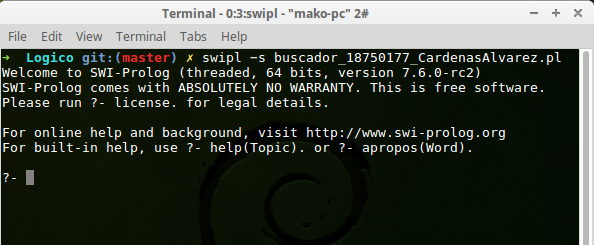
\includegraphics[width=1\textwidth]{ejecLinux.png}
    \caption{Compilación y ejecución del proyecto en entorno Linux}
    \label{fig:ejecLinux}
\end{figure}

Para terminar la ejecución del programa debe realizar la combinación de teclas:

\begin{lstlisting}[language=bash]
Ctrl + d
\end{lstlisting}

Esto interrumpe la ejecución del intérprete de SWI-Prolog y con ello la ejecución del programa.

\section {Entorno Windows}

Para poder realizar la compilación y ejecución del programa en un sistema operativo derivado de Windows es necesario tener instalado el compilador ``swipl'', asegúrese de tener instalada correctamente esta aplicación. Dicho lo anterior abra una terminal o consola del sistema y navegue en ella hasta el directorio del proyecto (utilizando el comando ``dir''), luego bastará con correr el siguiente comando:

\begin{lstlisting}[language=bash]
swipl -s buscador_18750177_CardenasAlvarez.pl
\end{lstlisting}

Se ejecutará el intérprete de SWI-Prolog con el sistema preparado para realizar consultas, la figura \ref{fig:ejecWin} muestra el proceso descrito.

\begin{figure}[H]
    \centering
    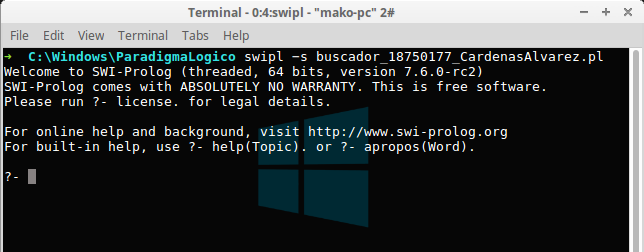
\includegraphics[width=1\textwidth]{ejecWin.png}
    \caption{Compilación y ejecución del proyecto en entorno Windows}
    \label{fig:ejecWin}
\end{figure}

Como puede observar el proceso es el mismo que en un sistema operativo derivado de Linux.

\chapter{Funcionalidades del programa}

Al ejecutar el programa es posible interactuar con él por medio del intérprete de SWI-Prolog, es decir puede hacer uso de las funcionalidades principales programadas en él, a continuación se detallan las funciones principales que puede realizar con el programa.

\section {Funciones principales}

Utilizando el intérprete el usuario puede realizar consultas al programa mediante los siguientes predicados:

\begin{description}[align=left]

\item [1.- singleTermQuery(Term, Result):] 
    El usuario puede consultar las ids de los documentos que contengan el término ``Term'', las ids serán retornadas mediante el parámetro ``Result''. 

\item [2.- bestMatch(Phrase, Result):]
    El usuario puede consultar las ids de los documentos que contengan al menos un término presente en la lista ``Phrase'', las ids serán retornadas mediante el parámetro ``Result''.

\item [3.- exactMatch(Phrase, Results):]
    El usuario puede consultar las ids de los documentos que contengan todos los términos presentes en la lista ``Phrase'', las ids serán retornadas mediante el parámetro ``Results''.

\item [4.- documents(Results, Documents):]
    El usuario puede consultar los títulos de los documentos que contengan las ids presentes en la lista ``Results'', los títulos serán retornados junto a su respectiva id mediante el parámetro ``Documents''.

\item [5.- numDocuments(Results, Count):]
    El usuario puede consultar los la cantidad de los documentos presentes en la lista ``Results'', la cantidad de elementos será retornada mediante el parámetro ``Count''.

\end{description}

A modo de ejemplo se sintetizan las consultas mencionadas anteriormente en la figura \ref{fig:test} donde pueden evidenciarse múltiples consultas con sus respectivos resultados.

\begin{figure}[H]
    \centering
    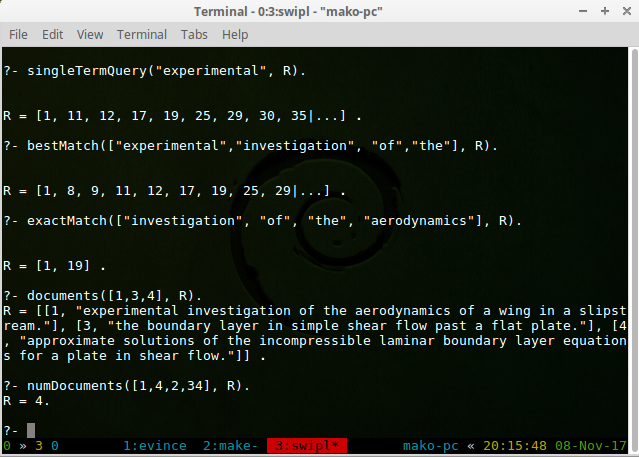
\includegraphics[width=1\textwidth]{test.png}
    \caption{Ejemplo de pruebas consultas en SWI-Prolog}
    \label{fig:test}
\end{figure}


\chapter{Control de flujo}

\section {Ejemplos e ilustraciones}

A modo de ejemplo se puede visualizar en la figura \ref{fig:success} como realizar una consulta exitosa a partir de una frase.

\begin{figure}[H]
    \centering
    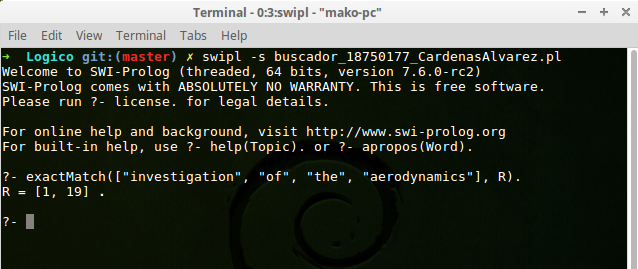
\includegraphics[width=1\textwidth]{success.png}
    \caption{Ejemplo de consulta exitosa}
    \label{fig:success}
\end{figure}

Por otro lado si se intenta realizar una operación el usuario sabrá que hubo un problema en su ejecución si el resultado es similar a lo que evidencia la figura \ref{fig:fail} en la que se muestra el intérprete reacciona ante un posible error.

\begin{figure}[H]
    \centering
    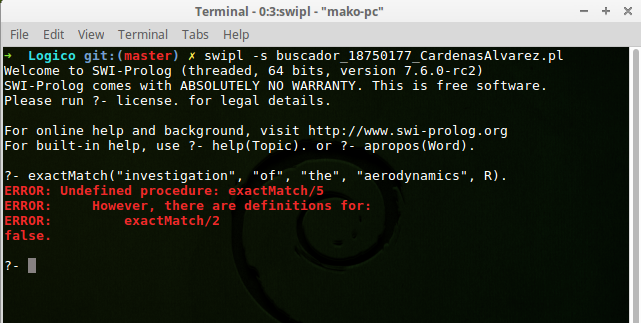
\includegraphics[width=1\textwidth]{fail.png}
    \caption{Ejemplo de consulta errónea}
    \label{fig:fail}
\end{figure}


\section {Control de errores}

Los errores mas frecuentes se presentan a continuación:

\begin{enumerate}

\item Asegúrese de que los datos ingresados sean correctos, si los parámetros de las funciones no son los esperados por las definiciones el programa arrojará un error. Para solucionarlo debe volver a realizar la consulta pero con los parámetros correctos, puede consultar en la sección ``Funciones principales'' los parámetros de las funciones.

\item Asegúrese de ejecutar el programa en el directorio del proyecto, si el directorio no es el correcto el programa arrojará un error. Para solucionarlo navegue en la terminal o consola hasta el directorio del proyecto, puede consultar en la sección ``Cómo compilar y ejecutar'' para mas información.

\item Use correctamente las cabeceras de las funciones, para utilizar las funciones definidas se deben llamar tal y como se muestra en los ejemplos, verifique la cantidad de parámetros, su tipificación y el nombre de la función.


\end{enumerate}

Si el usuario sigue las instrucciones especificadas en este documento el programa debe funcionar de manera correcta y sin errores.

\end{document}
